\documentclass{article}
\usepackage{amsmath}
\usepackage{graphicx}
\begin{document}
\title{Coordinate Geometry Unit Exam: Problem 43}
\author{Ana Bhattacharjee}
\date{\today}
\maketitle{}

\begin{center}
We simply plug in each point into the equation of the circle.
\begin{align}
  A (-1, 1) \\
  (-1)^2 + (1)^2 = 2 < 5
\end{align}
The point is within the circle.
\begin{align}
  B (-2, 1) \\
  (-2)^2 + (1)^2 = 5 = 5
\end{align}
the point is on the circle.
\begin{align}
  C (4, -8) \\
  (4)^2 + (-8)^2 = 16 + 64 > 5
\end{align}
The point is outside of the circle.
\par
\begin{figure}[!htbp]
  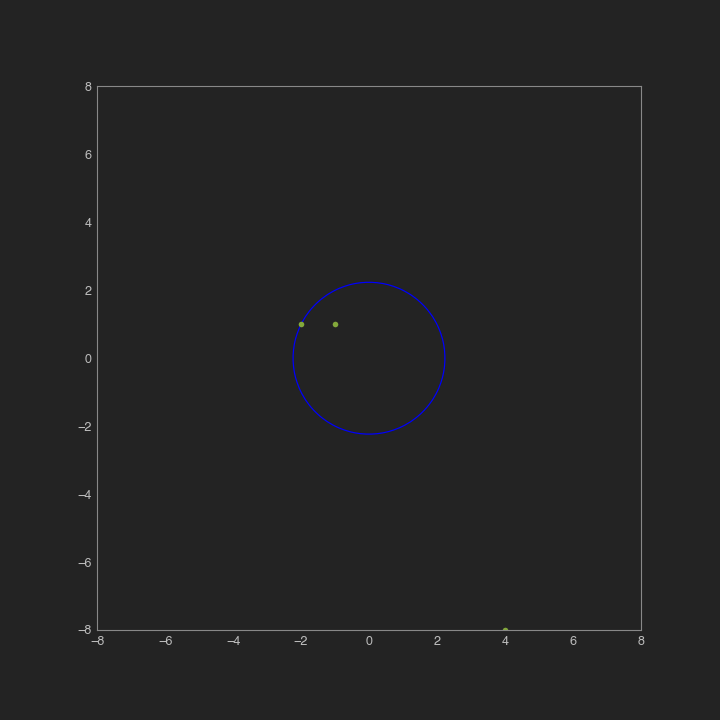
\includegraphics[width=1.0\columnwidth]{circle}
  \caption{Circle with Points}
\end{figure}
\end{center}
\end{document}
